%!TEX root=../paper.tex
The ChaCha stream cipher is a 256-bit stream cipher, designed by Bernstein in 2008~\cite{Ber:08}.
ChaCha based on the Salsa stream cipher has naturally a high-throughput performance on software platforms.
Compared to Salsa, ChaCha has better diffusion per round and conjecturally increasing resistance to cryptanalysis. 

\subsection{Encryption and Decryption}
The ChaCha encryption and decryption can have the same process in which the input data stream is encrypted or decrypted by chopping the input into 64-byte blocks and XOR-ing them with the 64-byte output blocks of the ChaCha block function. The block function processes on the ChaCha state matrix of $4\times4$ word (32-bit) elements to generate the 64-byte output block.
The ChaCha state matrix is initiated by a 4-word constant, an 8-word secret key, 4 words of counter/nonce. 
Note that the original ChaCha uses a 2-word nonce and a 2-word counter to allowing a practically unlimited amount of data to be encrypted while the IETF variant~\cite{RFC:18} increases the nonce size to 3 words, but reduces the counter size down to one word.
That limits the amount of encrypted data only up to 256 GB but helps the encryption more safely with a longer (key, nonce) pair. 
This paper adopts the IETF variant of which the initial state matrix is shown in (\ref{equ:bg:ChaChaMatix}.) %~\REFFIG{fig:bg:ChaChaMatix}.
The ChaCha process for encryption and decryption can be described as in Algorithm~\ref{alg::ChaCha::process}.

%\begin{figure}
%	\centering
%	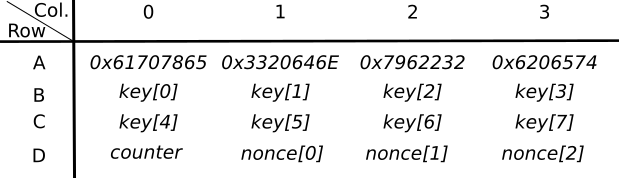
\includegraphics[scale=0.5]{figures/ChaChaState.png}
%	\caption{ChaCha Initiate State Matrix}
%	\vspace{-10pt}
%	\label{fig:bg:ChaChaMatix}
%\end{figure}
\begin{equation}
S=
\begin{pmatrix}
$61707865$ & $3320646E$ & $79622D32$ & $6B206574$ \\
key[$0$] & key[$1$]   & key[$2$]   & key[$3$] \\
key[$4$] & key[$5$]   & key[$6$]   & key[$7$] \\
counter  & nonce[$0$] & nonce[$1$] & nonce[$2$] \\
\end{pmatrix} 
\label{equ:bg:ChaChaMatix}
\end{equation}

\subsection{Block function}
ChaCha cipher family provides three variants which use different number
of operations performed on the state (i.e., $8$, $12$ or $20$ rounds). 
A larger number of rounds increases data diffusion and therefore more secure, but longer processing time. 
From now on, we focus on the ChaCha20 variant that executes $20$ rounds which alternately perform odd rounds and even rounds. The processed state matrix is, then, added to the input state matrix to result in the output state matrix. The operation of the block function is described in Algorithm~\ref{alg::ChaCha::block}.

\paragraph{Round function} Both of the odd and even rounds have 4 quarter rounds.
In the odd (column) round, the quarter rounds operate on four elements of the state matrix's columns.
While the quarter rounds of the even (diagonal) round operate on the diagonals of the state matrix.
For some implementations, one can view that a diagonal round can be equivalent to a column round, and vice versa, if the state matrix is rearranged (rotating the matrix's columns 1, 2, and 3) before the rounds. 

\paragraph{Quarter-Round function} A quarter round updates four state words of the state matrix as shown in~Algorithm~\ref{alg::ChaCha::quarterround}. 
The quarter round based on Add-Rotate-Xor (ARX) operations requires four sets of 32-bit Additions, Xors and  rotations operating on the state words. 
Each word is updated twice and affected by all four input words.

\begin{algorithm}
	\KwData  { 256-bit $Key$, 96-bit $Nonce$, L-bit $P$ 
	}
	\KwResult{ L-bit $C$
	}
	\BlankLine
	\KwFn{$\ALG{ChaChaProcess}( Key, Nonce, P )$}{
		/*Init state matrix*/ \;
		$S[0] \ASN \VERB{0x61707865}, S[1] \ASN \VERB{0x3320646e}$ \;
		$S[2] \ASN \VERB{0x79622d32}, S[3] \ASN \VERB{0x6b206574}$ \;
		$S[4..11] \ASN Key, S[13..15] \ASN Nonce$ \;
		/*Encrypting loop*/ \;
		\For{$i = 0$ {\bf upto} $\lceil\frac{L}{512}\rceil - 1$} {
			$S[12] \ASN i$ \;%\tcp{update counter} 
			$K_i \ASN \ALG {ChaChaBlock}( S )$ \; 
			$C_i \ASN K_i \XOR P_i$   \;%\tcp{perform encryption} 
		}
		$\KwRet{~C}$ \;
	}
	\caption{ChaCha Stream Cipher Process}
	\label{alg::ChaCha::process}
\end{algorithm}

\begin{algorithm}
	\KwData  { an input state matrix $S$ as an array of 16 32-bit state elements
	}
	\KwResult{ an output state matrix $K$ as an array of 16 32-bit state elements
	}
	\BlankLine
	\KwFn{$\ALG{ChaChaBlock}( S )$}{
%		/*copy the original state*/ \;
		$X \ASN S$ \;
		\For{$i = 1$ {\bf upto} $10$} {
			/*Odd Round*/ \;
			$\ALG{QuarterRound}( X[0],~X[4],~X[8],~X[12] )$ \; 
			$\ALG{QuarterRound}( X[1],~X[5],~X[9],~X[13] )$ \; 
			$\ALG{QuarterRound}( X[2],~X[6],~X[10],X[14] )$ \; 
			$\ALG{QuarterRound}( X[3],~X[7],~X[11],X[15] )$ \;  
			/*Even round*/ \;
			$\ALG{QuarterRound}( X[0],~X[5],~X[10],X[15] )$ \; 
			$\ALG{QuarterRound}( X[1],~X[6],~X[11],X[12] )$ \; 
			$\ALG{QuarterRound}( X[2],~X[7],~X[8]~,X[13] )$ \; 
			$\ALG{QuarterRound}( X[3],~X[4],~X[9]~,X[14] )$ \;  
		}
		$K \ASN X + S$ \;
		$\KwRet{~K}$ \;
	}
	\caption{ChaCha Block function}
	\label{alg::ChaCha::block}
\end{algorithm}

\begin{algorithm}
\KwData  { $A$, $B$, $C$, $D$ (32-bit state emelents).
}
\KwResult{ $A$, $B$, $C$, $D$ (Updated 32-bit state emelents).
}
\BlankLine
\KwFn{$\ALG{QuarterRound}( A, B, C, D )$}{
    /*Top half*/ \;
	$A \ASN A + B,~D \ASN D \XOR A,~D \ASN D \LRT 16$ \;
	$C \ASN C + D,~B \ASN B \XOR C,~B \ASN B \LRT 12$ \;
    /*Bottom half*/ \;
	$A \ASN A + B,~D \ASN D \XOR A,~D \ASN D \LRT  8$ \;
	$C \ASN C + D,~B \ASN B \XOR C,~B \ASN B \LRT  7$ \;
  $\KwRet{\TUPLE{ A, B, C, D }}$ \;
}
\caption{ChaCha Quarter Round}
\label{alg::ChaCha::quarterround}
\end{algorithm}
